%%% template.tex
%%%
%%% This LaTeX source document can be used as the basis for your technical
%%% paper or abstract. Intentionally stripped of annotation, the parameters
%%% and commands should be adjusted for your particular paper - title, 
%%% author, article DOI, etc.
%%% The accompanying ``template.annotated.tex'' provides copious annotation
%%% for the commands and parameters found in the source document. (The code
%%% is identical in ``template.tex'' and ``template.annotated.tex.'')

\documentclass[conference]{acmsiggraph}

\TOGonlineid{45678}
\TOGvolume{0}
\TOGnumber{0}
\TOGarticleDOI{1111111.2222222}
\TOGprojectURL{}
\TOGvideoURL{}
\TOGdataURL{}
\TOGcodeURL{}

\title{Shareable AI : How to get and share everybody's AI}

%%\author{Robert A. Smith\thanks{e-mail:rsmith@gmail.com}\\Smith Research}
\author{Jonathan Loquet - Lucas Tixier - Kevin Waththuhewa\\ESGI - Ecole Superieure de Genie Informatique, France}
\pdfauthor{Jonathan Loquet - Lucas Tixier - Kevin Waththuhewa}

\keywords{AI, video games, share}

\begin{document}

\teaser{
  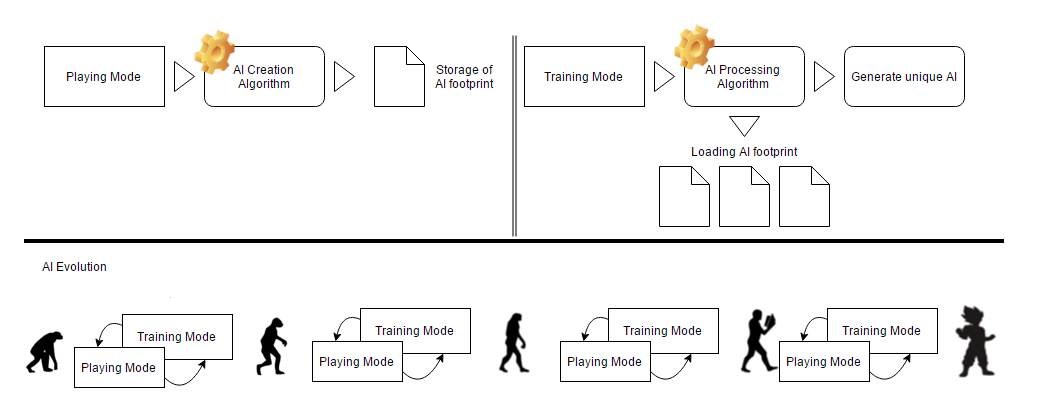
\includegraphics[height=1.5in]{images/ImagePaper}
  \caption{Shareable AI timeline, 2015}
}

\maketitle

%% Use this only if you're preparing a technical paper to be published in the 
%% ACM 'Transactions on Graphics' journal.

%%\TOGlinkslist

%% Required for all content. 

\copyrightspace

\section{Introduction}

%This paper propose a new way of playing with friends thanks to the machin learning.
Our goal is to allow player to access to someone else's artificial intelligence in order to play against an evolved AI. This system takes place in a small context like mini games. Each time a player will play to a mini games, he will create an AI in his image. This new AI will be share and anyone could download and play against it. 

This sharing system allow players AI not to be always the same, provide a way to see other people’s technique and also try to defeat the best players of the world.

\section{Annalyze, Train, Improve}

There is two mode that the player can choose. The first is the normal mode, this mode is the one that improve the shareable AI. The second one is the training mode that allow player to see what his weakness are and also how efficiently his AI is.
In the training mode, the player is confronted to his shareable AI, therefore he can understand what mistakes he made and also what he can change to make his shareable AI better. Then he can improve it in the normal mode.

Each game are very specific, therefore our system analyze each mini games in a different way. During this phase, all the player's logic and behavior is interpreted and update the shareable AI. Each mini games need a different number of steps to be analyzed. For instance imagine a mini game that consist in going through a labyrinth. The first step of the analysis is a simple path analyzer. In fact we just interpret all player's movement. Does the player always go forward ? Or does he just turn in the same direction all the time ? This player behaviour is interpreted and reflects the player's techniques and instinct.

The shareable AI is not a ghost of the player. For instance, when you will play against an other player's AI, this AI will not be the exact copy of the player behaviour. But it will be very influenced by it. The shareable AI is like a pupil and you are the teacher. You will give some tips to you shareable AI and he will apply it.

\section{AI File Structure}

We have different solution to store and read data
\begin{itemize}
	\item LUA → Looks like it exists but it seems to be kind of complicated to install
	\item XML → Unreal has a native class that seems to be easy to use on the C++
	\item JSON → We found a plugin downloadable and is unusable in blueprint
\end{itemize}

The datas are stored in a file, most likely in a XML file as we work with Unreal 4.
We create XML markers which correspond to various datas.
As our context is mini games, we have one AI per mini game for one player. Which means that each mini game have their own different datas.

So the data struct have a name/id for the game as the first node.
Then, the following node is the datas collected about the behaviour.
Maybe, some secondary node represent slices of time in order to determine the player behaviour at different step.

As the interpretation of the data is in the code according to the mini game, we just need to feed the AI with the datas so that the AI will behave in order to obtain approximately the same datas.
In order to avoid the AI to act the same way with the same datas, we add some random and some threshold (like more or less 10\% of a value to reach)

The AI of the player is updated according to the score he gets while playing. At the end of the game, the datas harvested are computed.
In order to have an evolution and not a complet reset of the behaviors, we have to smooth the different corresponding datas (like calculating an average value between the old and the new data).

In order to collect the datas, we have to pinpoint what is monitored in the action of the player.
Like, some action give the player a certain amount of point. And the more the player have points the more he has a good behavior in order to win.
At the end we look at the total score. Then the sub score to see where he got good mark and where not.
Maybe it would be good to keep 2 or 3 differentes behaviors having a great score.
%%\begin{figure}[ht]
%%  \centering
%%  \includegraphics[width=1.5in]{images/samplefigure}
%%  \caption{Sample illustration.}
%%\end{figure}

\bibliographystyle{acmsiggraph}
%%\bibliography{template}
\end{document}
